\documentclass[../main/report.tex]{subfiles}
\begin{document}

\chapter{GPU}

The GPU is at the heart of the Demolicious system.
Inspired by SIMD and SIMT architecture and programming models, the GPU architecture is named 'GhettoCUDA' in honor of NVIDIAs CUDA environment.\todo{cite this}

The GhettoCUDA architecture is highly parallel, in that it allows for a great number of threads to execute in parallel on multiple streaming processors.
A thread is the unit of execution, in essence a single procedure, that when correctly parameterized by run-time values allows for the transformation of a set of input data to a graphical representation to be visualized by the HDMI module.
A simple kernel, requiring no input, might be one that for each pixel in the framebuffer stores the color red.

The main design challenge in creating a GPU-inspired system is managing to saturate the memory bus as much as possible, changing memory access patterns from clustering together in time to a more spread-out pattern.
To facilitate this, the architecture allowing for multiple threads to execute on each streaming processor core, with a staggered start.
This design decision allows for a steady stream of load/store instructions without requiring a system stall as one waits for memory requests to return.

\section{Responsibilities}

The GPU has these responsibilities
\begin{enumerate}
  \item
    Receive instructions and constants from the CPU
  \item
    Handle kernel invocations from the CPU
  \item
    Write results to external SRAM
  \item
    Assert the 'computation finished' signal to the CPU
\end{enumerate}

\section{Architecture Overview}
\begin{figure}[H]
\centering
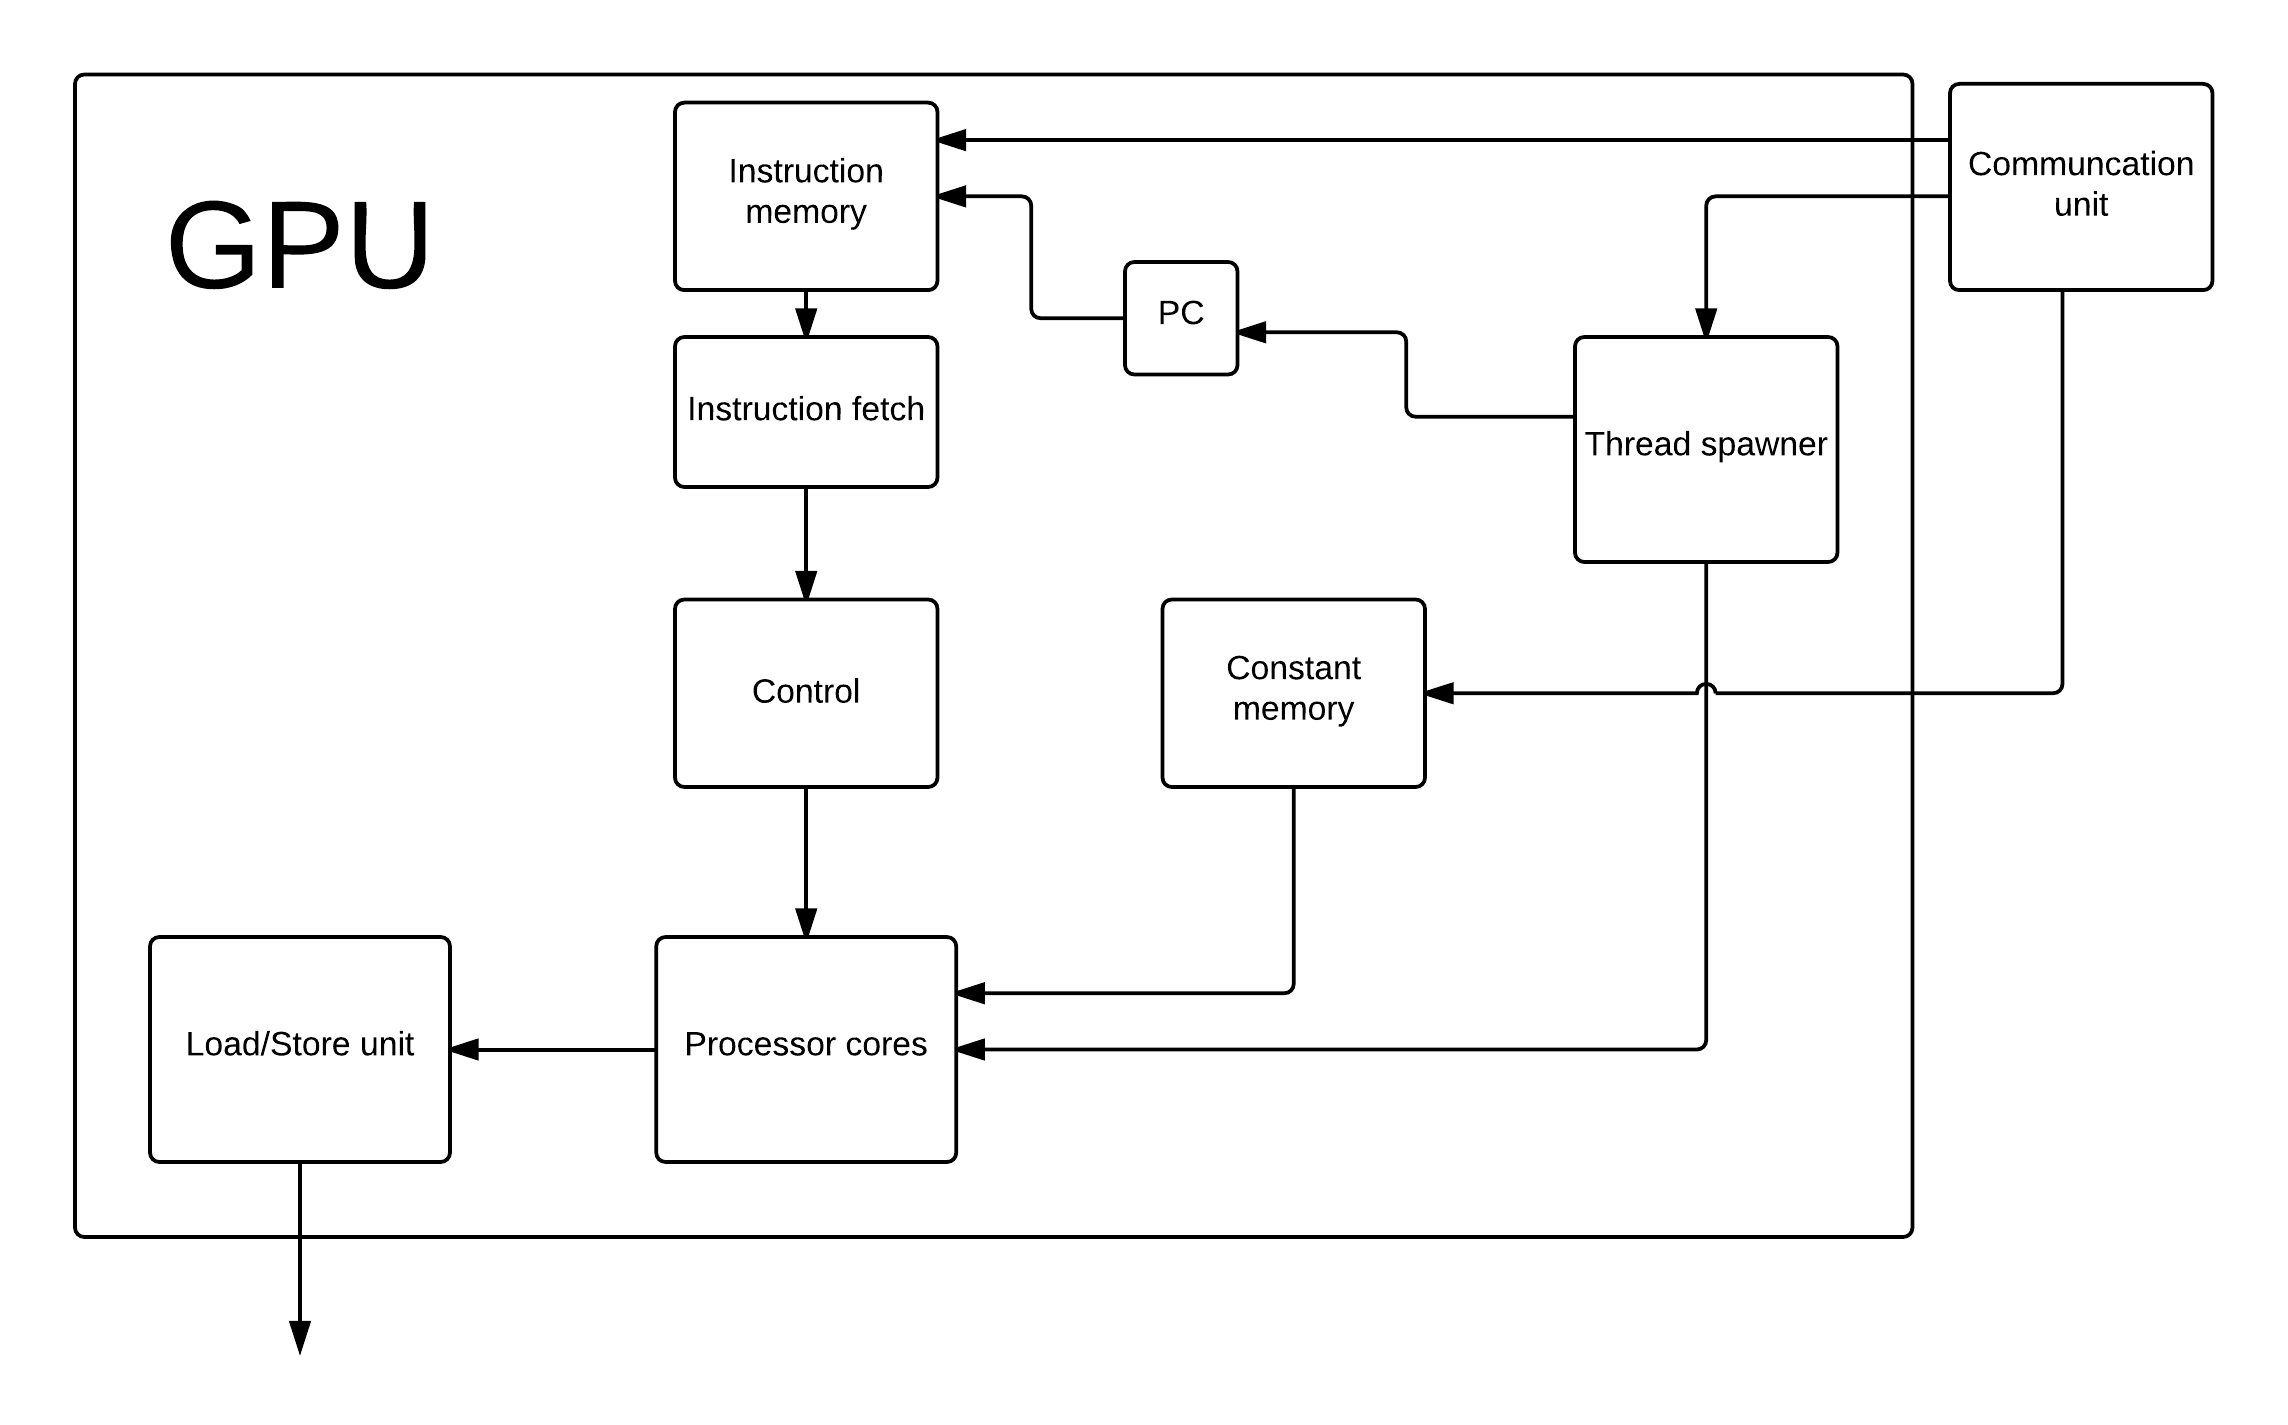
\includegraphics[width=\textwidth]{../gpu/diagrams/architecture_overview.png}
\caption{A high level overview of the GPU.}
\label{fig:architecture_overview}
\end{figure}
Figure \ref{fig:architecture_overview} presents a high level overview over the GPU.
The CPU issues commands to the communication unit in the GPU. Commands are launching a kernel, uploading kernels to the instruction memory, writing to the constant memory, and read/write to SRAM.
Instructions are fetched from the instruction memory and decoded by the control unit, which has the responsibility of setting the control signals for the instructions.
The processors load constants from the constant memory, and uses the load/store unit for accessing the data memory.


\section{Receiving a Kernel Call}
\begin{figure}[H]
\centering
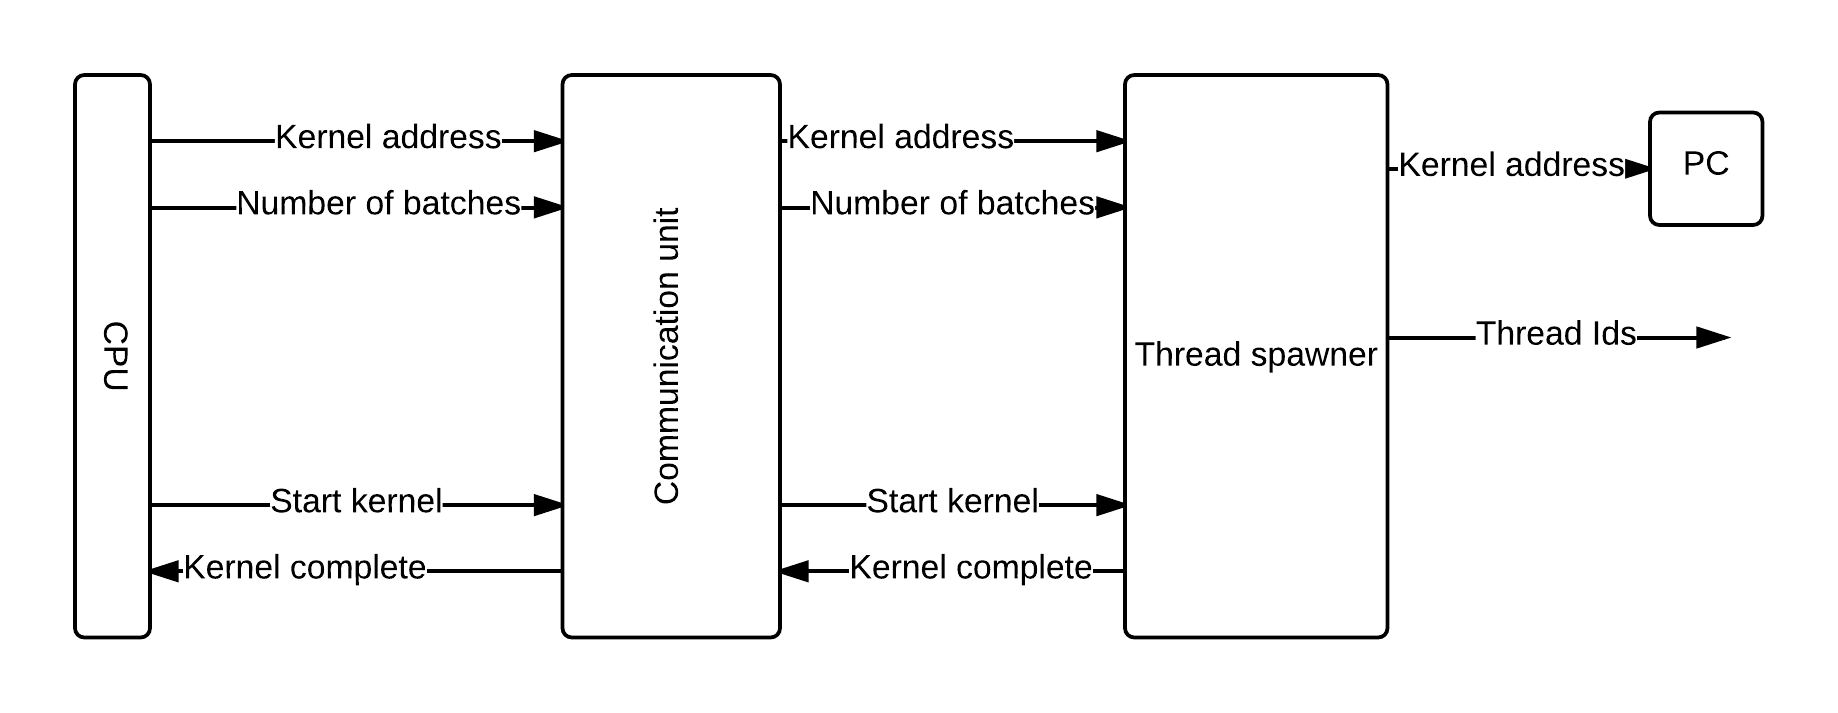
\includegraphics[width=\textwidth]{../gpu/diagrams/receiving_a_kernel_call.png}
\caption{Launching a kernel from the GPU's viewpoint.}
\label{fig:kernel_call}
\end{figure}

The communication unit is responsible for receiving kernel call requests from the CPU.
When a kernel call is received, the kernel launch signal is asserted.
A kernel call consists of the address of the kernel, and the number of threads to launch.

The kernel launch signals are forwarded to the thread spawner, which writes the kernel start address to the PC register, and starts distributing thread IDs to the processor cores. 
After holding the kernel launch signals high, the communication unit has completed its role in launching the kernel.
When the kernel completes executing, the thread spawner asserts the kernel done signal, and the communication unit forwards the signal to the CPU, indicating that the kernel call has completed.


\section{Running a Kernel}
Once the thread spawner has been initiated by the communication unit, the kernel runs to completion without intervention by the CPU. 
When a kernel run starts, the thread spawner assigns thread IDs to each warp in the barrel.
After the initial IDs have been assigned the GPU enters normal execution.
\begin{figure}[H]
	\centering
	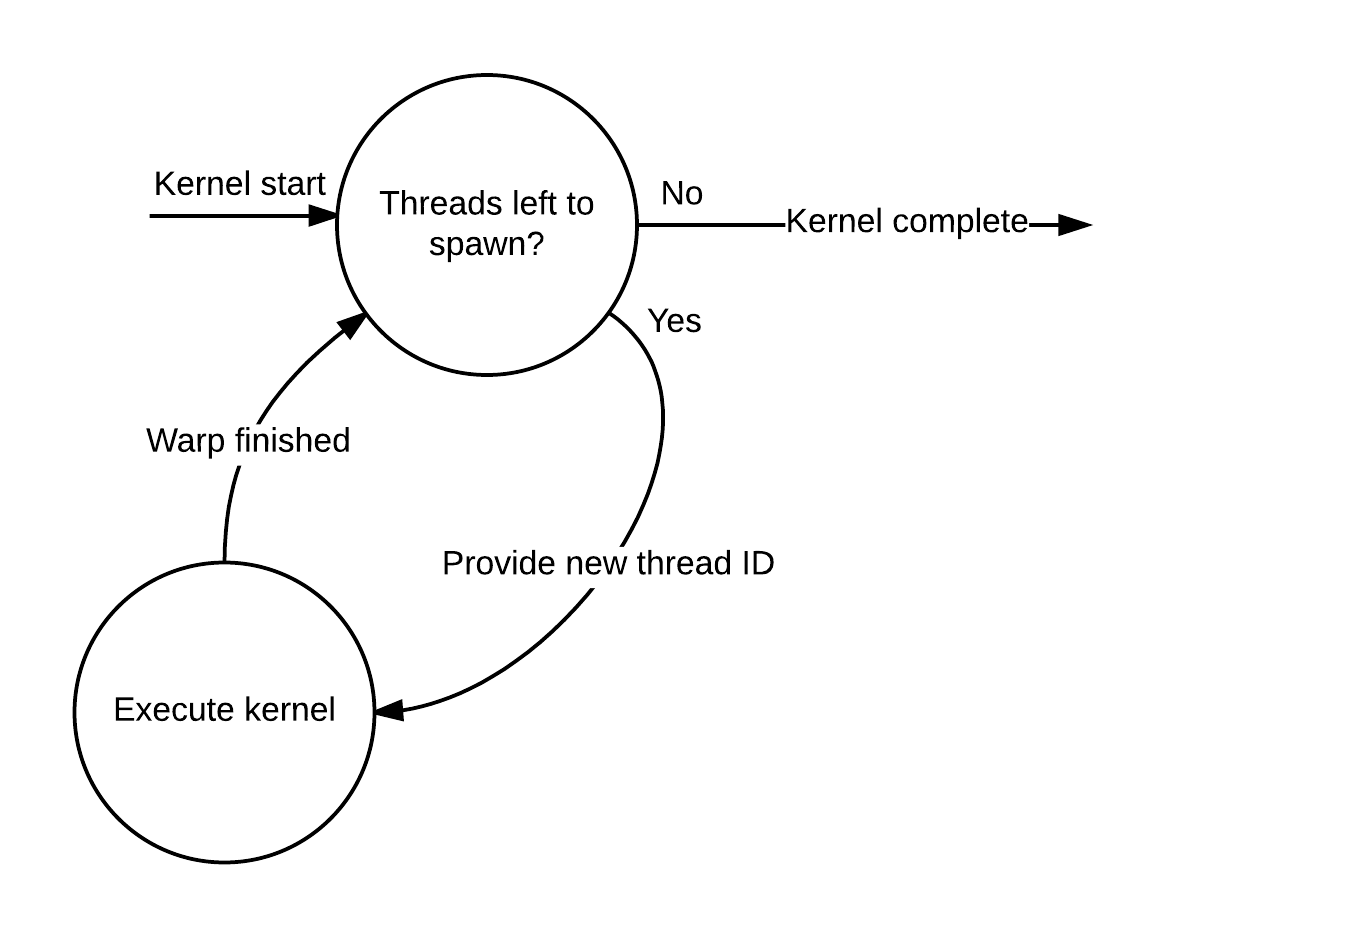
\includegraphics[width=0.9\textwidth]{../gpu/diagrams/kernel_run_state_machine.png}
	\caption{The GPU's internal state during kernel execution.}
	\label{fig:kernel_run_state_machine}
\end{figure}
A normal kernel execution can be represented by the state machine in figure \ref{fig:kernel_run_state_machine}.
During the kernel execution stage the threads in a warp execute the same instructions, until the control unit encounters a \emph{finished} instruction.
Upon receiving a \emph{finished} instruction the control unit asserts the \emph{finished} signal alerting the thread spawner that a new warp has to be spawned.
The thread spawner keeps track of the number of threads awaiting launch.
When the thread spawner receives a \emph{finished} instruction and no more warps are awaiting launch, the kernel complete signal is asserted, and the kernel run has completed.


\section{Module Details}

\subfile{../gpu/core.tex}

\subfile{../gpu/thread-spawner.tex}

\subfile{../gpu/regdir.tex}

\subfile{../gpu/sram.tex}

\subfile{../gpu/lsu.tex}

\subfile{../gpu/hdmi.tex}

\end{document}
